\documentclass[1p]{elsarticle_modified}
%\bibliographystyle{elsarticle-num}

%\usepackage[colorlinks]{hyperref}
%\usepackage{abbrmath_seonhwa} %\Abb, \Ascr, \Acal ,\Abf, \Afrak
\usepackage{amsfonts}
\usepackage{amssymb}
\usepackage{amsmath}
\usepackage{amsthm}
\usepackage{scalefnt}
\usepackage{amsbsy}
\usepackage{kotex}
\usepackage{caption}
\usepackage{subfig}
\usepackage{color}
\usepackage{graphicx}
\usepackage{xcolor} %% white, black, red, green, blue, cyan, magenta, yellow
\usepackage{float}
\usepackage{setspace}
\usepackage{hyperref}

\usepackage{tikz}
\usetikzlibrary{arrows}

\usepackage{multirow}
\usepackage{array} % fixed length table
\usepackage{hhline}

%%%%%%%%%%%%%%%%%%%%%
\makeatletter
\renewcommand*\env@matrix[1][\arraystretch]{%
	\edef\arraystretch{#1}%
	\hskip -\arraycolsep
	\let\@ifnextchar\new@ifnextchar
	\array{*\c@MaxMatrixCols c}}
\makeatother %https://tex.stackexchange.com/questions/14071/how-can-i-increase-the-line-spacing-in-a-matrix
%%%%%%%%%%%%%%%

\usepackage[normalem]{ulem}

\newcommand{\msout}[1]{\ifmmode\text{\sout{\ensuremath{#1}}}\else\sout{#1}\fi}
%SOURCE: \msout is \stkout macro in https://tex.stackexchange.com/questions/20609/strikeout-in-math-mode

\newcommand{\cancel}[1]{
	\ifmmode
	{\color{red}\msout{#1}}
	\else
	{\color{red}\sout{#1}}
	\fi
}

\newcommand{\add}[1]{
	{\color{blue}\uwave{#1}}
}

\newcommand{\replace}[2]{
	\ifmmode
	{\color{red}\msout{#1}}{\color{blue}\uwave{#2}}
	\else
	{\color{red}\sout{#1}}{\color{blue}\uwave{#2}}
	\fi
}

\newcommand{\Sol}{\mathcal{S}} %segment
\newcommand{\D}{D} %diagram
\newcommand{\A}{\mathcal{A}} %arc


%%%%%%%%%%%%%%%%%%%%%%%%%%%%%5 test

\def\sl{\operatorname{\textup{SL}}(2,\Cbb)}
\def\psl{\operatorname{\textup{PSL}}(2,\Cbb)}
\def\quan{\mkern 1mu \triangleright \mkern 1mu}

\theoremstyle{definition}
\newtheorem{thm}{Theorem}[section]
\newtheorem{prop}[thm]{Proposition}
\newtheorem{lem}[thm]{Lemma}
\newtheorem{ques}[thm]{Question}
\newtheorem{cor}[thm]{Corollary}
\newtheorem{defn}[thm]{Definition}
\newtheorem{exam}[thm]{Example}
\newtheorem{rmk}[thm]{Remark}
\newtheorem{alg}[thm]{Algorithm}

\newcommand{\I}{\sqrt{-1}}
\begin{document}

%\begin{frontmatter}
%
%\title{Boundary parabolic representations of knots up to 8 crossings}
%
%%% Group authors per affiliation:
%\author{Yunhi Cho} 
%\address{Department of Mathematics, University of Seoul, Seoul, Korea}
%\ead{yhcho@uos.ac.kr}
%
%
%\author{Seonhwa Kim} %\fnref{s_kim}}
%\address{Center for Geometry and Physics, Institute for Basic Science, Pohang, 37673, Korea}
%\ead{ryeona17@ibs.re.kr}
%
%\author{Hyuk Kim}
%\address{Department of Mathematical Sciences, Seoul National University, Seoul 08826, Korea}
%\ead{hyukkim@snu.ac.kr}
%
%\author{Seokbeom Yoon}
%\address{Department of Mathematical Sciences, Seoul National University, Seoul, 08826,  Korea}
%\ead{sbyoon15@snu.ac.kr}
%
%\begin{abstract}
%We find all boundary parabolic representation of knots up to 8 crossings.
%
%\end{abstract}
%\begin{keyword}
%    \MSC[2010] 57M25 
%\end{keyword}
%
%\end{frontmatter}

%\linenumbers
%\tableofcontents
%
\newcommand\colored[1]{\textcolor{white}{\rule[-0.35ex]{0.8em}{1.4ex}}\kern-0.8em\color{red} #1}%
%\newcommand\colored[1]{\textcolor{white}{ #1}\kern-2.17ex	\textcolor{white}{ #1}\kern-1.81ex	\textcolor{white}{ #1}\kern-2.15ex\color{red}#1	}

{\Large $\underline{12a_{0889}~(K12a_{0889})}$}

\setlength{\tabcolsep}{10pt}
\renewcommand{\arraystretch}{1.6}
\vspace{1cm}\begin{tabular}{m{100pt}>{\centering\arraybackslash}m{274pt}}
\multirow{5}{120pt}{
	\centering
	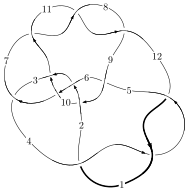
\includegraphics[width=112pt]{../../../GIT/diagram.site/Diagrams/png/1690_12a_0889.png}\\
\ \ \ A knot diagram\footnotemark}&
\allowdisplaybreaks
\textbf{Linearized knot diagam} \\
\cline{2-2}
 &
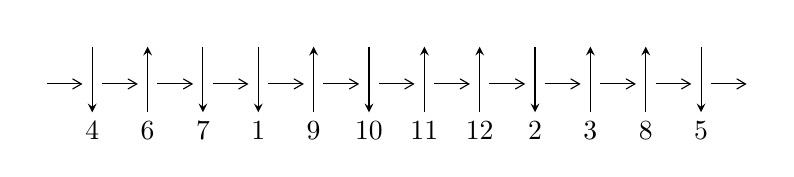
\begin{tikzpicture}[x=20pt, y=17pt]
	% nodes
	\node (C0) at (0, 0) {};
	\node (C1) at (1, 0) {};
	\node (C1U) at (1, +1) {};
	\node (C1D) at (1, -1) {4};

	\node (C2) at (2, 0) {};
	\node (C2U) at (2, +1) {};
	\node (C2D) at (2, -1) {6};

	\node (C3) at (3, 0) {};
	\node (C3U) at (3, +1) {};
	\node (C3D) at (3, -1) {7};

	\node (C4) at (4, 0) {};
	\node (C4U) at (4, +1) {};
	\node (C4D) at (4, -1) {1};

	\node (C5) at (5, 0) {};
	\node (C5U) at (5, +1) {};
	\node (C5D) at (5, -1) {9};

	\node (C6) at (6, 0) {};
	\node (C6U) at (6, +1) {};
	\node (C6D) at (6, -1) {10};

	\node (C7) at (7, 0) {};
	\node (C7U) at (7, +1) {};
	\node (C7D) at (7, -1) {11};

	\node (C8) at (8, 0) {};
	\node (C8U) at (8, +1) {};
	\node (C8D) at (8, -1) {12};

	\node (C9) at (9, 0) {};
	\node (C9U) at (9, +1) {};
	\node (C9D) at (9, -1) {2};

	\node (C10) at (10, 0) {};
	\node (C10U) at (10, +1) {};
	\node (C10D) at (10, -1) {3};

	\node (C11) at (11, 0) {};
	\node (C11U) at (11, +1) {};
	\node (C11D) at (11, -1) {8};

	\node (C12) at (12, 0) {};
	\node (C12U) at (12, +1) {};
	\node (C12D) at (12, -1) {5};
	\node (C13) at (13, 0) {};

	% arrows
	\draw[->,>={angle 60}]
	(C0) edge (C1) (C1) edge (C2) (C2) edge (C3) (C3) edge (C4) (C4) edge (C5) (C5) edge (C6) (C6) edge (C7) (C7) edge (C8) (C8) edge (C9) (C9) edge (C10) (C10) edge (C11) (C11) edge (C12) (C12) edge (C13) ;	\draw[->,>=stealth]
	(C1U) edge (C1D) (C2D) edge (C2U) (C3U) edge (C3D) (C4U) edge (C4D) (C5D) edge (C5U) (C6U) edge (C6D) (C7D) edge (C7U) (C8D) edge (C8U) (C9U) edge (C9D) (C10D) edge (C10U) (C11D) edge (C11U) (C12U) edge (C12D) ;
	\end{tikzpicture} \\
\hhline{~~} \\& 
\textbf{Solving Sequence} \\ \cline{2-2} 
 &
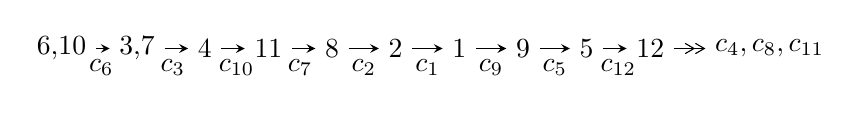
\begin{tikzpicture}[x=23pt, y=7pt]
	% node
	\node (A0) at (-1/8, 0) {6,10};
	\node (A1) at (17/16, 0) {3,7};
	\node (A2) at (17/8, 0) {4};
	\node (A3) at (25/8, 0) {11};
	\node (A4) at (33/8, 0) {8};
	\node (A5) at (41/8, 0) {2};
	\node (A6) at (49/8, 0) {1};
	\node (A7) at (57/8, 0) {9};
	\node (A8) at (65/8, 0) {5};
	\node (A9) at (73/8, 0) {12};
	\node (C1) at (1/2, -1) {$c_{6}$};
	\node (C2) at (13/8, -1) {$c_{3}$};
	\node (C3) at (21/8, -1) {$c_{10}$};
	\node (C4) at (29/8, -1) {$c_{7}$};
	\node (C5) at (37/8, -1) {$c_{2}$};
	\node (C6) at (45/8, -1) {$c_{1}$};
	\node (C7) at (53/8, -1) {$c_{9}$};
	\node (C8) at (61/8, -1) {$c_{5}$};
	\node (C9) at (69/8, -1) {$c_{12}$};
	\node (A10) at (11, 0) {$c_{4},c_{8},c_{11}$};

	% edge
	\draw[->,>=stealth]	
	(A0) edge (A1) (A1) edge (A2) (A2) edge (A3) (A3) edge (A4) (A4) edge (A5) (A5) edge (A6) (A6) edge (A7) (A7) edge (A8) (A8) edge (A9) ;
	\draw[->>,>={angle 60}]	
	(A9) edge (A10);
\end{tikzpicture} \\ 

\end{tabular} \\

\footnotetext{
The image of knot diagram is generated by the software ``\textbf{Draw programme}" developed by Andrew Bartholomew(\url{http://www.layer8.co.uk/maths/draw/index.htm\#Running-draw}), where we modified some parts for our purpose(\url{https://github.com/CATsTAILs/LinksPainter}).
}\phantom \\ \newline 
\centering \textbf{Ideals for irreducible components\footnotemark of $X_{\text{par}}$} 
 
\begin{align*}
I^u_{1}&=\langle 
1.44342\times10^{568} u^{109}-5.63890\times10^{568} u^{108}+\cdots+2.52973\times10^{568} b-7.41395\times10^{568},\\
\phantom{I^u_{1}}&\phantom{= \langle  }-5.01819\times10^{569} u^{109}+1.42633\times10^{570} u^{108}+\cdots+1.26486\times10^{569} a-8.15947\times10^{570},\\
\phantom{I^u_{1}}&\phantom{= \langle  }u^{110}-3 u^{109}+\cdots+21 u+1\rangle \\
I^u_{2}&=\langle 
-2.15930\times10^{15} u^{20}-9.88518\times10^{15} u^{19}+\cdots+1.08985\times10^{15} b-4.65481\times10^{15},\\
\phantom{I^u_{2}}&\phantom{= \langle  }-4.00480\times10^{15} u^{20}-1.80755\times10^{16} u^{19}+\cdots+1.08985\times10^{15} a-7.18818\times10^{15},\;u^{21}+5 u^{20}+\cdots+5 u+1\rangle \\
I^u_{3}&=\langle 
b,\;- u^5-4 u^4-5 u^3-2 u^2+a-2 u-3,\;u^6+3 u^5+2 u^4- u^3+u^2+2 u-1\rangle \\
\\
\end{align*}
\raggedright * 3 irreducible components of $\dim_{\mathbb{C}}=0$, with total 137 representations.\\
\footnotetext{All coefficients of polynomials are rational numbers. But the coefficients are sometimes approximated in decimal forms when there is not enough margin.}
\newpage
\renewcommand{\arraystretch}{1}
\centering \section*{I. $I^u_{1}= \langle 1.44\times10^{568} u^{109}-5.64\times10^{568} u^{108}+\cdots+2.53\times10^{568} b-7.41\times10^{568},\;-5.02\times10^{569} u^{109}+1.43\times10^{570} u^{108}+\cdots+1.26\times10^{569} a-8.16\times10^{570},\;u^{110}-3 u^{109}+\cdots+21 u+1 \rangle$}
\flushleft \textbf{(i) Arc colorings}\\
\begin{tabular}{m{7pt} m{180pt} m{7pt} m{180pt} }
\flushright $a_{6}=$&$\begin{pmatrix}1\\0\end{pmatrix}$ \\
\flushright $a_{10}=$&$\begin{pmatrix}0\\u\end{pmatrix}$ \\
\flushright $a_{3}=$&$\begin{pmatrix}3.96738 u^{109}-11.2766 u^{108}+\cdots+710.062 u+64.5087\\-0.570582 u^{109}+2.22905 u^{108}+\cdots+8.69317 u+2.93073\end{pmatrix}$ \\
\flushright $a_{7}=$&$\begin{pmatrix}1\\u^2\end{pmatrix}$ \\
\flushright $a_{4}=$&$\begin{pmatrix}4.01600 u^{109}-11.7395 u^{108}+\cdots+684.265 u+60.9524\\-0.359351 u^{109}+1.46248 u^{108}+\cdots+15.3016 u+3.24774\end{pmatrix}$ \\
\flushright $a_{11}=$&$\begin{pmatrix}-7.92618 u^{109}+25.6136 u^{108}+\cdots-555.057 u-43.9460\\-1.48877 u^{109}+4.66015 u^{108}+\cdots-143.849 u-11.6428\end{pmatrix}$ \\
\flushright $a_{8}=$&$\begin{pmatrix}-2.52216 u^{109}+6.77640 u^{108}+\cdots-613.962 u-68.2999\\-0.392391 u^{109}+1.13085 u^{108}+\cdots-78.1210 u-8.94244\end{pmatrix}$ \\
\flushright $a_{2}=$&$\begin{pmatrix}4.53796 u^{109}-13.5056 u^{108}+\cdots+701.369 u+61.5780\\-0.570582 u^{109}+2.22905 u^{108}+\cdots+8.69317 u+2.93073\end{pmatrix}$ \\
\flushright $a_{1}=$&$\begin{pmatrix}7.32097 u^{109}-22.4072 u^{108}+\cdots+873.765 u+74.0818\\0.953125 u^{109}-3.04274 u^{108}+\cdots+83.6563 u+7.91593\end{pmatrix}$ \\
\flushright $a_{9}=$&$\begin{pmatrix}-6.06911 u^{109}+20.0584 u^{108}+\cdots-322.474 u-24.0997\\-0.368302 u^{109}+0.895009 u^{108}+\cdots-86.7341 u-8.20350\end{pmatrix}$ \\
\flushright $a_{5}=$&$\begin{pmatrix}6.02161 u^{109}-18.1467 u^{108}+\cdots+821.524 u+72.9777\\0.00590647 u^{109}+0.241512 u^{108}+\cdots+48.2897 u+6.22933\end{pmatrix}$ \\
\flushright $a_{12}=$&$\begin{pmatrix}9.98424 u^{109}-30.9702 u^{108}+\cdots+1068.56 u+89.7856\\1.79589 u^{109}-5.80409 u^{108}+\cdots+145.185 u+12.5127\end{pmatrix}$\\&\end{tabular}
\flushleft \textbf{(ii) Obstruction class $= -1$}\\~\\
\flushleft \textbf{(iii) Cusp Shapes $= 23.7845 u^{109}-78.8398 u^{108}+\cdots+1380.90 u+90.0800$}\\~\\
\newpage\renewcommand{\arraystretch}{1}
\flushleft \textbf{(iv) u-Polynomials at the component}\newline \\
\begin{tabular}{m{50pt}|m{274pt}}
Crossings & \hspace{64pt}u-Polynomials at each crossing \\
\hline $$\begin{aligned}c_{1},c_{4},c_{12}\end{aligned}$$&$\begin{aligned}
&u^{110}+3 u^{109}+\cdots-62 u+7
\end{aligned}$\\
\hline $$\begin{aligned}c_{2}\end{aligned}$$&$\begin{aligned}
&u^{110}-6 u^{108}+\cdots-1248 u+64
\end{aligned}$\\
\hline $$\begin{aligned}c_{3}\end{aligned}$$&$\begin{aligned}
&u^{110}+18 u^{108}+\cdots-5982 u+511
\end{aligned}$\\
\hline $$\begin{aligned}c_{5}\end{aligned}$$&$\begin{aligned}
&u^{110}- u^{109}+\cdots+127044378 u+11982227
\end{aligned}$\\
\hline $$\begin{aligned}c_{6}\end{aligned}$$&$\begin{aligned}
&u^{110}-3 u^{109}+\cdots+21 u+1
\end{aligned}$\\
\hline $$\begin{aligned}c_{7},c_{8},c_{11}\end{aligned}$$&$\begin{aligned}
&u^{110}-4 u^{109}+\cdots+146 u+11
\end{aligned}$\\
\hline $$\begin{aligned}c_{9}\end{aligned}$$&$\begin{aligned}
&u^{110}-2 u^{108}+\cdots-434 u+115
\end{aligned}$\\
\hline $$\begin{aligned}c_{10}\end{aligned}$$&$\begin{aligned}
&u^{110}+u^{109}+\cdots+4063 u+1795
\end{aligned}$\\
\hline
\end{tabular}\\~\\
\newpage\renewcommand{\arraystretch}{1}
\flushleft \textbf{(v) Riley Polynomials at the component}\newline \\
\begin{tabular}{m{50pt}|m{274pt}}
Crossings & \hspace{64pt}Riley Polynomials at each crossing \\
\hline $$\begin{aligned}c_{1},c_{4},c_{12}\end{aligned}$$&$\begin{aligned}
&y^{110}+115 y^{109}+\cdots-694 y+49
\end{aligned}$\\
\hline $$\begin{aligned}c_{2}\end{aligned}$$&$\begin{aligned}
&y^{110}-12 y^{109}+\cdots-844800 y+4096
\end{aligned}$\\
\hline $$\begin{aligned}c_{3}\end{aligned}$$&$\begin{aligned}
&y^{110}+36 y^{109}+\cdots-9724346 y+261121
\end{aligned}$\\
\hline $$\begin{aligned}c_{5}\end{aligned}$$&$\begin{aligned}
&y^{110}-59 y^{109}+\cdots-8074941417464332 y+143573763879529
\end{aligned}$\\
\hline $$\begin{aligned}c_{6}\end{aligned}$$&$\begin{aligned}
&y^{110}-15 y^{109}+\cdots-183 y+1
\end{aligned}$\\
\hline $$\begin{aligned}c_{7},c_{8},c_{11}\end{aligned}$$&$\begin{aligned}
&y^{110}-128 y^{109}+\cdots-17642 y+121
\end{aligned}$\\
\hline $$\begin{aligned}c_{9}\end{aligned}$$&$\begin{aligned}
&y^{110}-4 y^{109}+\cdots-38396 y+13225
\end{aligned}$\\
\hline $$\begin{aligned}c_{10}\end{aligned}$$&$\begin{aligned}
&y^{110}-27 y^{109}+\cdots-181138189 y+3222025
\end{aligned}$\\
\hline
\end{tabular}\\~\\
\newpage\flushleft \textbf{(vi) Complex Volumes and Cusp Shapes}
$$\begin{array}{c|c|c}  
\text{Solutions to }I^u_{1}& \I (\text{vol} + \sqrt{-1}CS) & \text{Cusp shape}\\
 \hline 
\begin{aligned}
u &= \phantom{-}0.774572 + 0.632471 I \\
a &= -0.89220 + 1.52122 I \\
b &= -0.548053 + 0.137687 I\end{aligned}
 & \phantom{-}7.93768 - 5.25317 I & \phantom{-0.000000 } 0 \\ \hline\begin{aligned}
u &= \phantom{-}0.774572 - 0.632471 I \\
a &= -0.89220 - 1.52122 I \\
b &= -0.548053 - 0.137687 I\end{aligned}
 & \phantom{-}7.93768 + 5.25317 I & \phantom{-0.000000 } 0 \\ \hline\begin{aligned}
u &= -0.560346 + 0.853408 I \\
a &= \phantom{-}0.047334 - 1.169540 I \\
b &= -0.535513 - 0.176348 I\end{aligned}
 & \phantom{-}1.56438 + 2.47087 I & \phantom{-0.000000 } 0 \\ \hline\begin{aligned}
u &= -0.560346 - 0.853408 I \\
a &= \phantom{-}0.047334 + 1.169540 I \\
b &= -0.535513 + 0.176348 I\end{aligned}
 & \phantom{-}1.56438 - 2.47087 I & \phantom{-0.000000 } 0 \\ \hline\begin{aligned}
u &= \phantom{-}0.124231 + 0.956021 I \\
a &= -0.332111 + 0.655043 I \\
b &= -1.24931 + 1.41822 I\end{aligned}
 & \phantom{-}14.9970 - 6.5880 I & \phantom{-0.000000 } 0 \\ \hline\begin{aligned}
u &= \phantom{-}0.124231 - 0.956021 I \\
a &= -0.332111 - 0.655043 I \\
b &= -1.24931 - 1.41822 I\end{aligned}
 & \phantom{-}14.9970 + 6.5880 I & \phantom{-0.000000 } 0 \\ \hline\begin{aligned}
u &= -0.715385 + 0.756555 I \\
a &= \phantom{-}0.877620 + 0.541968 I \\
b &= \phantom{-}1.141200 - 0.158237 I\end{aligned}
 & \phantom{-}8.97543 - 0.77350 I & \phantom{-0.000000 } 0 \\ \hline\begin{aligned}
u &= -0.715385 - 0.756555 I \\
a &= \phantom{-}0.877620 - 0.541968 I \\
b &= \phantom{-}1.141200 + 0.158237 I\end{aligned}
 & \phantom{-}8.97543 + 0.77350 I & \phantom{-0.000000 } 0 \\ \hline\begin{aligned}
u &= -0.310378 + 0.905410 I \\
a &= -0.015555 - 0.706392 I \\
b &= -1.14977 - 1.14634 I\end{aligned}
 & \phantom{-}8.12852 + 4.99064 I & \phantom{-0.000000 } 0 \\ \hline\begin{aligned}
u &= -0.310378 - 0.905410 I \\
a &= -0.015555 + 0.706392 I \\
b &= -1.14977 + 1.14634 I\end{aligned}
 & \phantom{-}8.12852 - 4.99064 I & \phantom{-0.000000 } 0\\
 \hline 
 \end{array}$$\newpage$$\begin{array}{c|c|c}  
\text{Solutions to }I^u_{1}& \I (\text{vol} + \sqrt{-1}CS) & \text{Cusp shape}\\
 \hline 
\begin{aligned}
u &= \phantom{-}0.591904 + 0.870733 I \\
a &= \phantom{-}0.130086 + 1.177850 I \\
b &= -1.08337 + 0.94972 I\end{aligned}
 & \phantom{-}8.72354 - 3.03179 I & \phantom{-0.000000 } 0 \\ \hline\begin{aligned}
u &= \phantom{-}0.591904 - 0.870733 I \\
a &= \phantom{-}0.130086 - 1.177850 I \\
b &= -1.08337 - 0.94972 I\end{aligned}
 & \phantom{-}8.72354 + 3.03179 I & \phantom{-0.000000 } 0 \\ \hline\begin{aligned}
u &= \phantom{-}0.838495 + 0.390871 I \\
a &= \phantom{-}0.889756 + 0.699588 I \\
b &= -0.089294 + 0.460614 I\end{aligned}
 & \phantom{-}2.44031 - 0.26635 I & \phantom{-0.000000 } 0 \\ \hline\begin{aligned}
u &= \phantom{-}0.838495 - 0.390871 I \\
a &= \phantom{-}0.889756 - 0.699588 I \\
b &= -0.089294 - 0.460614 I\end{aligned}
 & \phantom{-}2.44031 + 0.26635 I & \phantom{-0.000000 } 0 \\ \hline\begin{aligned}
u &= \phantom{-}0.476011 + 0.782871 I \\
a &= \phantom{-}0.494024 - 0.502108 I \\
b &= \phantom{-}1.50207 - 0.99579 I\end{aligned}
 & \phantom{-}7.79132 - 3.43252 I & \phantom{-0.000000 } 0 \\ \hline\begin{aligned}
u &= \phantom{-}0.476011 - 0.782871 I \\
a &= \phantom{-}0.494024 + 0.502108 I \\
b &= \phantom{-}1.50207 + 0.99579 I\end{aligned}
 & \phantom{-}7.79132 + 3.43252 I & \phantom{-0.000000 } 0 \\ \hline\begin{aligned}
u &= \phantom{-}0.475946 + 0.976502 I \\
a &= -0.24106 - 1.59534 I \\
b &= \phantom{-}0.873118 - 0.085672 I\end{aligned}
 & \phantom{-}16.7347 - 7.7979 I & \phantom{-0.000000 } 0 \\ \hline\begin{aligned}
u &= \phantom{-}0.475946 - 0.976502 I \\
a &= -0.24106 + 1.59534 I \\
b &= \phantom{-}0.873118 + 0.085672 I\end{aligned}
 & \phantom{-}16.7347 + 7.7979 I & \phantom{-0.000000 } 0 \\ \hline\begin{aligned}
u &= -0.677755 + 0.612424 I \\
a &= \phantom{-}0.053848 + 0.679869 I \\
b &= \phantom{-}1.083870 + 0.901794 I\end{aligned}
 & \phantom{-}0.92636 + 3.37225 I & \phantom{-0.000000 } 0 \\ \hline\begin{aligned}
u &= -0.677755 - 0.612424 I \\
a &= \phantom{-}0.053848 - 0.679869 I \\
b &= \phantom{-}1.083870 - 0.901794 I\end{aligned}
 & \phantom{-}0.92636 - 3.37225 I & \phantom{-0.000000 } 0\\
 \hline 
 \end{array}$$\newpage$$\begin{array}{c|c|c}  
\text{Solutions to }I^u_{1}& \I (\text{vol} + \sqrt{-1}CS) & \text{Cusp shape}\\
 \hline 
\begin{aligned}
u &= -0.945732 + 0.546364 I \\
a &= \phantom{-}0.070342 + 0.756458 I \\
b &= \phantom{-}1.045450 + 0.883608 I\end{aligned}
 & \phantom{-}0.95831 + 3.29223 I & \phantom{-0.000000 } 0 \\ \hline\begin{aligned}
u &= -0.945732 - 0.546364 I \\
a &= \phantom{-}0.070342 - 0.756458 I \\
b &= \phantom{-}1.045450 - 0.883608 I\end{aligned}
 & \phantom{-}0.95831 - 3.29223 I & \phantom{-0.000000 } 0 \\ \hline\begin{aligned}
u &= \phantom{-}0.891739\phantom{ +0.000000I} \\
a &= \phantom{-}2.12201\phantom{ +0.000000I} \\
b &= \phantom{-}0.428233\phantom{ +0.000000I}\end{aligned}
 & \phantom{-}4.79546\phantom{ +0.000000I} & \phantom{-0.000000 } 0 \\ \hline\begin{aligned}
u &= -0.732004 + 0.848914 I \\
a &= -0.02463 - 1.55659 I \\
b &= -1.23288 - 0.92476 I\end{aligned}
 & \phantom{-}16.4324 + 2.2483 I & \phantom{-0.000000 } 0 \\ \hline\begin{aligned}
u &= -0.732004 - 0.848914 I \\
a &= -0.02463 + 1.55659 I \\
b &= -1.23288 + 0.92476 I\end{aligned}
 & \phantom{-}16.4324 - 2.2483 I & \phantom{-0.000000 } 0 \\ \hline\begin{aligned}
u &= -0.828689 + 0.765989 I \\
a &= -0.451776 - 0.468277 I \\
b &= \phantom{-}0.260810 - 0.056998 I\end{aligned}
 & \phantom{-}2.75921 + 2.65033 I & \phantom{-0.000000 } 0 \\ \hline\begin{aligned}
u &= -0.828689 - 0.765989 I \\
a &= -0.451776 + 0.468277 I \\
b &= \phantom{-}0.260810 + 0.056998 I\end{aligned}
 & \phantom{-}2.75921 - 2.65033 I & \phantom{-0.000000 } 0 \\ \hline\begin{aligned}
u &= -0.785131\phantom{ +0.000000I} \\
a &= \phantom{-}1.46415\phantom{ +0.000000I} \\
b &= \phantom{-}0.0826449\phantom{ +0.000000I}\end{aligned}
 & -1.06875\phantom{ +0.000000I} & \phantom{-0.000000 } 0 \\ \hline\begin{aligned}
u &= -0.661247 + 0.408466 I \\
a &= \phantom{-}1.83442 - 1.69581 I \\
b &= -0.596866 - 0.927607 I\end{aligned}
 & \phantom{-}12.5489 + 8.8816 I & \phantom{-0.000000 } 0 \\ \hline\begin{aligned}
u &= -0.661247 - 0.408466 I \\
a &= \phantom{-}1.83442 + 1.69581 I \\
b &= -0.596866 + 0.927607 I\end{aligned}
 & \phantom{-}12.5489 - 8.8816 I & \phantom{-0.000000 } 0\\
 \hline 
 \end{array}$$\newpage$$\begin{array}{c|c|c}  
\text{Solutions to }I^u_{1}& \I (\text{vol} + \sqrt{-1}CS) & \text{Cusp shape}\\
 \hline 
\begin{aligned}
u &= -1.106860 + 0.536656 I \\
a &= -0.401468 - 0.704362 I \\
b &= -0.153166 - 0.706136 I\end{aligned}
 & \phantom{-}2.53752 + 2.32422 I & \phantom{-0.000000 } 0 \\ \hline\begin{aligned}
u &= -1.106860 - 0.536656 I \\
a &= -0.401468 + 0.704362 I \\
b &= -0.153166 + 0.706136 I\end{aligned}
 & \phantom{-}2.53752 - 2.32422 I & \phantom{-0.000000 } 0 \\ \hline\begin{aligned}
u &= \phantom{-}0.654893 + 0.375970 I \\
a &= -0.281669 + 1.103070 I \\
b &= \phantom{-}0.59368 + 1.30161 I\end{aligned}
 & \phantom{-}4.93851 - 5.82307 I & \phantom{-0.000000 } 0 \\ \hline\begin{aligned}
u &= \phantom{-}0.654893 - 0.375970 I \\
a &= -0.281669 - 1.103070 I \\
b &= \phantom{-}0.59368 - 1.30161 I\end{aligned}
 & \phantom{-}4.93851 + 5.82307 I & \phantom{-0.000000 } 0 \\ \hline\begin{aligned}
u &= -1.157250 + 0.509604 I \\
a &= -0.935247 - 0.035605 I \\
b &= -1.278610 + 0.474048 I\end{aligned}
 & \phantom{-}15.0541 + 3.2345 I & \phantom{-0.000000 } 0 \\ \hline\begin{aligned}
u &= -1.157250 - 0.509604 I \\
a &= -0.935247 + 0.035605 I \\
b &= -1.278610 - 0.474048 I\end{aligned}
 & \phantom{-}15.0541 - 3.2345 I & \phantom{-0.000000 } 0 \\ \hline\begin{aligned}
u &= \phantom{-}0.975718 + 0.808390 I \\
a &= \phantom{-}0.213090 - 1.081970 I \\
b &= \phantom{-}1.12209 - 0.94361 I\end{aligned}
 & \phantom{-}1.06256 - 5.18407 I & \phantom{-0.000000 } 0 \\ \hline\begin{aligned}
u &= \phantom{-}0.975718 - 0.808390 I \\
a &= \phantom{-}0.213090 + 1.081970 I \\
b &= \phantom{-}1.12209 + 0.94361 I\end{aligned}
 & \phantom{-}1.06256 + 5.18407 I & \phantom{-0.000000 } 0 \\ \hline\begin{aligned}
u &= \phantom{-}1.011570 + 0.788569 I \\
a &= -0.823264 - 0.221926 I \\
b &= \phantom{-}0.232331 - 0.660204 I\end{aligned}
 & \phantom{-}8.66796 - 0.78567 I & \phantom{-0.000000 } 0 \\ \hline\begin{aligned}
u &= \phantom{-}1.011570 - 0.788569 I \\
a &= -0.823264 + 0.221926 I \\
b &= \phantom{-}0.232331 + 0.660204 I\end{aligned}
 & \phantom{-}8.66796 + 0.78567 I & \phantom{-0.000000 } 0\\
 \hline 
 \end{array}$$\newpage$$\begin{array}{c|c|c}  
\text{Solutions to }I^u_{1}& \I (\text{vol} + \sqrt{-1}CS) & \text{Cusp shape}\\
 \hline 
\begin{aligned}
u &= -0.992265 + 0.832307 I \\
a &= \phantom{-}0.338617 + 1.315790 I \\
b &= \phantom{-}1.32936 + 1.00820 I\end{aligned}
 & \phantom{-}8.35865 + 6.84750 I & \phantom{-0.000000 } 0 \\ \hline\begin{aligned}
u &= -0.992265 - 0.832307 I \\
a &= \phantom{-}0.338617 - 1.315790 I \\
b &= \phantom{-}1.32936 - 1.00820 I\end{aligned}
 & \phantom{-}8.35865 - 6.84750 I & \phantom{-0.000000 } 0 \\ \hline\begin{aligned}
u &= -0.290577 + 1.294510 I \\
a &= -0.446532 + 0.767605 I \\
b &= \phantom{-}0.781428 - 0.075730 I\end{aligned}
 & \phantom{-}8.52066 + 3.04058 I & \phantom{-0.000000 } 0 \\ \hline\begin{aligned}
u &= -0.290577 - 1.294510 I \\
a &= -0.446532 - 0.767605 I \\
b &= \phantom{-}0.781428 + 0.075730 I\end{aligned}
 & \phantom{-}8.52066 - 3.04058 I & \phantom{-0.000000 } 0 \\ \hline\begin{aligned}
u &= \phantom{-}0.585661 + 1.201620 I \\
a &= -0.163568 + 0.494662 I \\
b &= -0.642186 - 0.037791 I\end{aligned}
 & \phantom{-}1.98677 + 2.15796 I & \phantom{-0.000000 } 0 \\ \hline\begin{aligned}
u &= \phantom{-}0.585661 - 1.201620 I \\
a &= -0.163568 - 0.494662 I \\
b &= -0.642186 + 0.037791 I\end{aligned}
 & \phantom{-}1.98677 - 2.15796 I & \phantom{-0.000000 } 0 \\ \hline\begin{aligned}
u &= \phantom{-}1.218800 + 0.550512 I \\
a &= \phantom{-}0.451453 - 0.351078 I \\
b &= \phantom{-}0.627504 - 0.232141 I\end{aligned}
 & \phantom{-}1.088670 - 0.212814 I & \phantom{-0.000000 } 0 \\ \hline\begin{aligned}
u &= \phantom{-}1.218800 - 0.550512 I \\
a &= \phantom{-}0.451453 + 0.351078 I \\
b &= \phantom{-}0.627504 + 0.232141 I\end{aligned}
 & \phantom{-}1.088670 + 0.212814 I & \phantom{-0.000000 } 0 \\ \hline\begin{aligned}
u &= \phantom{-}1.266440 + 0.438516 I \\
a &= -0.444059 + 0.139336 I \\
b &= -1.48742 + 0.18860 I\end{aligned}
 & \phantom{-}6.81283 + 0.18653 I & \phantom{-0.000000 } 0 \\ \hline\begin{aligned}
u &= \phantom{-}1.266440 - 0.438516 I \\
a &= -0.444059 - 0.139336 I \\
b &= -1.48742 - 0.18860 I\end{aligned}
 & \phantom{-}6.81283 - 0.18653 I & \phantom{-0.000000 } 0\\
 \hline 
 \end{array}$$\newpage$$\begin{array}{c|c|c}  
\text{Solutions to }I^u_{1}& \I (\text{vol} + \sqrt{-1}CS) & \text{Cusp shape}\\
 \hline 
\begin{aligned}
u &= -0.658241 + 0.031826 I \\
a &= \phantom{-}0.394930 + 0.351966 I \\
b &= -0.719040 + 0.317896 I\end{aligned}
 & -1.407700 + 0.051950 I & -7.32066 + 0.87113 I \\ \hline\begin{aligned}
u &= -0.658241 - 0.031826 I \\
a &= \phantom{-}0.394930 - 0.351966 I \\
b &= -0.719040 - 0.317896 I\end{aligned}
 & -1.407700 - 0.051950 I & -7.32066 - 0.87113 I \\ \hline\begin{aligned}
u &= -0.639006 + 0.142930 I \\
a &= -1.01394 + 3.27755 I \\
b &= \phantom{-}0.264559 + 1.069070 I\end{aligned}
 & \phantom{-}4.82862 + 3.59852 I & -2.49071 - 6.47593 I \\ \hline\begin{aligned}
u &= -0.639006 - 0.142930 I \\
a &= -1.01394 - 3.27755 I \\
b &= \phantom{-}0.264559 - 1.069070 I\end{aligned}
 & \phantom{-}4.82862 - 3.59852 I & -2.49071 + 6.47593 I \\ \hline\begin{aligned}
u &= \phantom{-}0.503809 + 0.382796 I \\
a &= \phantom{-}2.19844 + 0.92750 I \\
b &= -0.728895 + 0.615188 I\end{aligned}
 & \phantom{-}5.78183 - 5.82433 I & \phantom{-}2.76550 + 9.85542 I \\ \hline\begin{aligned}
u &= \phantom{-}0.503809 - 0.382796 I \\
a &= \phantom{-}2.19844 - 0.92750 I \\
b &= -0.728895 - 0.615188 I\end{aligned}
 & \phantom{-}5.78183 + 5.82433 I & \phantom{-}2.76550 - 9.85542 I \\ \hline\begin{aligned}
u &= \phantom{-}0.599522\phantom{ +0.000000I} \\
a &= \phantom{-}1.09470\phantom{ +0.000000I} \\
b &= \phantom{-}0.509246\phantom{ +0.000000I}\end{aligned}
 & \phantom{-}1.20815\phantom{ +0.000000I} & \phantom{-}8.23520\phantom{ +0.000000I} \\ \hline\begin{aligned}
u &= \phantom{-}0.940720 + 1.038890 I \\
a &= -0.258390 + 0.915531 I \\
b &= -0.453797 + 0.622087 I\end{aligned}
 & \phantom{-}7.19253 - 5.38461 I & \phantom{-0.000000 } 0 \\ \hline\begin{aligned}
u &= \phantom{-}0.940720 - 1.038890 I \\
a &= -0.258390 - 0.915531 I \\
b &= -0.453797 - 0.622087 I\end{aligned}
 & \phantom{-}7.19253 + 5.38461 I & \phantom{-0.000000 } 0 \\ \hline\begin{aligned}
u &= -0.530334 + 0.260982 I \\
a &= -0.35708 - 1.59712 I \\
b &= \phantom{-}0.77505 - 2.06037 I\end{aligned}
 & \phantom{-}13.0946 + 8.0575 I & \phantom{-}1.85904 - 10.14716 I\\
 \hline 
 \end{array}$$\newpage$$\begin{array}{c|c|c}  
\text{Solutions to }I^u_{1}& \I (\text{vol} + \sqrt{-1}CS) & \text{Cusp shape}\\
 \hline 
\begin{aligned}
u &= -0.530334 - 0.260982 I \\
a &= -0.35708 + 1.59712 I \\
b &= \phantom{-}0.77505 + 2.06037 I\end{aligned}
 & \phantom{-}13.0946 - 8.0575 I & \phantom{-}1.85904 + 10.14716 I \\ \hline\begin{aligned}
u &= \phantom{-}0.551499 + 0.202743 I \\
a &= -0.06841 - 2.08947 I \\
b &= \phantom{-}0.482359 - 1.142180 I\end{aligned}
 & -0.68842 - 2.45858 I & -2.82743 - 12.79099 I \\ \hline\begin{aligned}
u &= \phantom{-}0.551499 - 0.202743 I \\
a &= -0.06841 + 2.08947 I \\
b &= \phantom{-}0.482359 + 1.142180 I\end{aligned}
 & -0.68842 + 2.45858 I & -2.82743 + 12.79099 I \\ \hline\begin{aligned}
u &= -1.07049 + 0.95663 I \\
a &= \phantom{-}0.185131 + 0.691196 I \\
b &= \phantom{-}0.639211 + 0.760069 I\end{aligned}
 & -1.01440 + 3.57337 I & \phantom{-0.000000 } 0 \\ \hline\begin{aligned}
u &= -1.07049 - 0.95663 I \\
a &= \phantom{-}0.185131 - 0.691196 I \\
b &= \phantom{-}0.639211 - 0.760069 I\end{aligned}
 & -1.01440 - 3.57337 I & \phantom{-0.000000 } 0 \\ \hline\begin{aligned}
u &= -0.77761 + 1.21084 I \\
a &= -0.534344 - 0.449709 I \\
b &= -0.853078 + 0.209963 I\end{aligned}
 & \phantom{-}9.25940 - 5.46029 I & \phantom{-0.000000 } 0 \\ \hline\begin{aligned}
u &= -0.77761 - 1.21084 I \\
a &= -0.534344 + 0.449709 I \\
b &= -0.853078 - 0.209963 I\end{aligned}
 & \phantom{-}9.25940 + 5.46029 I & \phantom{-0.000000 } 0 \\ \hline\begin{aligned}
u &= \phantom{-}0.537860 + 0.113065 I \\
a &= \phantom{-}0.34732 - 1.46044 I \\
b &= -0.463002 - 1.318780 I\end{aligned}
 & -1.32056 - 2.31790 I & -8.22376 + 9.76978 I \\ \hline\begin{aligned}
u &= \phantom{-}0.537860 - 0.113065 I \\
a &= \phantom{-}0.34732 + 1.46044 I \\
b &= -0.463002 + 1.318780 I\end{aligned}
 & -1.32056 + 2.31790 I & -8.22376 - 9.76978 I \\ \hline\begin{aligned}
u &= \phantom{-}0.92147 + 1.12188 I \\
a &= \phantom{-}0.098895 - 0.858374 I \\
b &= \phantom{-}0.596369 - 1.099270 I\end{aligned}
 & \phantom{-}4.05554 - 5.99285 I & \phantom{-0.000000 } 0\\
 \hline 
 \end{array}$$\newpage$$\begin{array}{c|c|c}  
\text{Solutions to }I^u_{1}& \I (\text{vol} + \sqrt{-1}CS) & \text{Cusp shape}\\
 \hline 
\begin{aligned}
u &= \phantom{-}0.92147 - 1.12188 I \\
a &= \phantom{-}0.098895 + 0.858374 I \\
b &= \phantom{-}0.596369 + 1.099270 I\end{aligned}
 & \phantom{-}4.05554 + 5.99285 I & \phantom{-0.000000 } 0 \\ \hline\begin{aligned}
u &= \phantom{-}1.46526 + 0.06585 I \\
a &= -0.498390 + 0.371200 I \\
b &= -0.501537 + 0.613741 I\end{aligned}
 & \phantom{-}5.49251 + 1.87089 I & \phantom{-0.000000 } 0 \\ \hline\begin{aligned}
u &= \phantom{-}1.46526 - 0.06585 I \\
a &= -0.498390 - 0.371200 I \\
b &= -0.501537 - 0.613741 I\end{aligned}
 & \phantom{-}5.49251 - 1.87089 I & \phantom{-0.000000 } 0 \\ \hline\begin{aligned}
u &= -1.12400 + 0.94748 I \\
a &= -0.315673 - 1.094540 I \\
b &= -1.34237 - 0.99895 I\end{aligned}
 & \phantom{-}8.1642 + 13.0472 I & \phantom{-0.000000 } 0 \\ \hline\begin{aligned}
u &= -1.12400 - 0.94748 I \\
a &= -0.315673 + 1.094540 I \\
b &= -1.34237 + 0.99895 I\end{aligned}
 & \phantom{-}8.1642 - 13.0472 I & \phantom{-0.000000 } 0 \\ \hline\begin{aligned}
u &= \phantom{-}1.13720 + 0.95650 I \\
a &= -0.197715 + 0.921183 I \\
b &= -1.17583 + 0.87305 I\end{aligned}
 & \phantom{-}0.56405 - 9.77507 I & \phantom{-0.000000 } 0 \\ \hline\begin{aligned}
u &= \phantom{-}1.13720 - 0.95650 I \\
a &= -0.197715 - 0.921183 I \\
b &= -1.17583 - 0.87305 I\end{aligned}
 & \phantom{-}0.56405 + 9.77507 I & \phantom{-0.000000 } 0 \\ \hline\begin{aligned}
u &= -0.502519 + 0.108029 I \\
a &= \phantom{-}0.18397 + 2.04925 I \\
b &= -0.25502 + 2.34163 I\end{aligned}
 & \phantom{-}5.42423 + 3.37899 I & -9.68824 - 6.26167 I \\ \hline\begin{aligned}
u &= -0.502519 - 0.108029 I \\
a &= \phantom{-}0.18397 - 2.04925 I \\
b &= -0.25502 - 2.34163 I\end{aligned}
 & \phantom{-}5.42423 - 3.37899 I & -9.68824 + 6.26167 I \\ \hline\begin{aligned}
u &= \phantom{-}0.487910 + 0.157981 I \\
a &= -1.61676 - 2.24024 I \\
b &= \phantom{-}0.416359 - 0.793132 I\end{aligned}
 & -1.04722 - 2.44814 I & -10.34845 + 9.07272 I\\
 \hline 
 \end{array}$$\newpage$$\begin{array}{c|c|c}  
\text{Solutions to }I^u_{1}& \I (\text{vol} + \sqrt{-1}CS) & \text{Cusp shape}\\
 \hline 
\begin{aligned}
u &= \phantom{-}0.487910 - 0.157981 I \\
a &= -1.61676 + 2.24024 I \\
b &= \phantom{-}0.416359 + 0.793132 I\end{aligned}
 & -1.04722 + 2.44814 I & -10.34845 - 9.07272 I \\ \hline\begin{aligned}
u &= -0.311773 + 0.363570 I \\
a &= \phantom{-}2.18479 + 0.87316 I \\
b &= -1.042800 - 0.172901 I\end{aligned}
 & \phantom{-}6.35083 + 1.43301 I & \phantom{-}8.05925 - 0.03819 I \\ \hline\begin{aligned}
u &= -0.311773 - 0.363570 I \\
a &= \phantom{-}2.18479 - 0.87316 I \\
b &= -1.042800 + 0.172901 I\end{aligned}
 & \phantom{-}6.35083 - 1.43301 I & \phantom{-}8.05925 + 0.03819 I \\ \hline\begin{aligned}
u &= \phantom{-}0.95715 + 1.18988 I \\
a &= -0.066184 + 0.804498 I \\
b &= -0.62708 + 1.32672 I\end{aligned}
 & \phantom{-}9.82782 - 6.51847 I & \phantom{-0.000000 } 0 \\ \hline\begin{aligned}
u &= \phantom{-}0.95715 - 1.18988 I \\
a &= -0.066184 - 0.804498 I \\
b &= -0.62708 - 1.32672 I\end{aligned}
 & \phantom{-}9.82782 + 6.51847 I & \phantom{-0.000000 } 0 \\ \hline\begin{aligned}
u &= -0.386570 + 0.271191 I \\
a &= \phantom{-}0.86298 + 3.49150 I \\
b &= \phantom{-}0.162485 + 0.818563 I\end{aligned}
 & \phantom{-}3.63818 + 2.84038 I & \phantom{-}0.92503 - 6.05029 I \\ \hline\begin{aligned}
u &= -0.386570 - 0.271191 I \\
a &= \phantom{-}0.86298 - 3.49150 I \\
b &= \phantom{-}0.162485 - 0.818563 I\end{aligned}
 & \phantom{-}3.63818 - 2.84038 I & \phantom{-}0.92503 + 6.05029 I \\ \hline\begin{aligned}
u &= -1.16827 + 1.00540 I \\
a &= -0.092294 - 0.645658 I \\
b &= -1.041720 - 0.639340 I\end{aligned}
 & -0.45195 + 4.75197 I & \phantom{-0.000000 } 0 \\ \hline\begin{aligned}
u &= -1.16827 - 1.00540 I \\
a &= -0.092294 + 0.645658 I \\
b &= -1.041720 + 0.639340 I\end{aligned}
 & -0.45195 - 4.75197 I & \phantom{-0.000000 } 0 \\ \hline\begin{aligned}
u &= -1.16474 + 1.06625 I \\
a &= \phantom{-}0.234664 + 0.993604 I \\
b &= \phantom{-}1.34481 + 1.02397 I\end{aligned}
 & \phantom{-}15.2715 + 17.6049 I & \phantom{-0.000000 } 0\\
 \hline 
 \end{array}$$\newpage$$\begin{array}{c|c|c}  
\text{Solutions to }I^u_{1}& \I (\text{vol} + \sqrt{-1}CS) & \text{Cusp shape}\\
 \hline 
\begin{aligned}
u &= -1.16474 - 1.06625 I \\
a &= \phantom{-}0.234664 - 0.993604 I \\
b &= \phantom{-}1.34481 - 1.02397 I\end{aligned}
 & \phantom{-}15.2715 - 17.6049 I & \phantom{-0.000000 } 0 \\ \hline\begin{aligned}
u &= \phantom{-}0.170612 + 0.337681 I \\
a &= \phantom{-}1.03643 - 2.29648 I \\
b &= -1.67443 - 0.27296 I\end{aligned}
 & \phantom{-}14.1811 + 1.2153 I & \phantom{-}11.26046 + 0.21873 I \\ \hline\begin{aligned}
u &= \phantom{-}0.170612 - 0.337681 I \\
a &= \phantom{-}1.03643 + 2.29648 I \\
b &= -1.67443 + 0.27296 I\end{aligned}
 & \phantom{-}14.1811 - 1.2153 I & \phantom{-}11.26046 - 0.21873 I \\ \hline\begin{aligned}
u &= \phantom{-}1.19603 + 1.10006 I \\
a &= \phantom{-}0.139764 - 0.851353 I \\
b &= \phantom{-}1.23014 - 0.82756 I\end{aligned}
 & \phantom{-}7.0682 - 13.1651 I & \phantom{-0.000000 } 0 \\ \hline\begin{aligned}
u &= \phantom{-}1.19603 - 1.10006 I \\
a &= \phantom{-}0.139764 + 0.851353 I \\
b &= \phantom{-}1.23014 + 0.82756 I\end{aligned}
 & \phantom{-}7.0682 + 13.1651 I & \phantom{-0.000000 } 0 \\ \hline\begin{aligned}
u &= -1.10362 + 1.20410 I \\
a &= -0.160490 - 0.593138 I \\
b &= -0.665528 - 0.924470 I\end{aligned}
 & \phantom{-}3.20052 + 5.24080 I & \phantom{-0.000000 } 0 \\ \hline\begin{aligned}
u &= -1.10362 - 1.20410 I \\
a &= -0.160490 + 0.593138 I \\
b &= -0.665528 + 0.924470 I\end{aligned}
 & \phantom{-}3.20052 - 5.24080 I & \phantom{-0.000000 } 0 \\ \hline\begin{aligned}
u &= -0.99443 + 1.42886 I \\
a &= \phantom{-}0.451569 + 0.333754 I \\
b &= \phantom{-}0.738648 - 0.347544 I\end{aligned}
 & \phantom{-}16.0502 - 8.9937 I & \phantom{-0.000000 } 0 \\ \hline\begin{aligned}
u &= -0.99443 - 1.42886 I \\
a &= \phantom{-}0.451569 - 0.333754 I \\
b &= \phantom{-}0.738648 + 0.347544 I\end{aligned}
 & \phantom{-}16.0502 + 8.9937 I & \phantom{-0.000000 } 0 \\ \hline\begin{aligned}
u &= -1.28221 + 1.22669 I \\
a &= \phantom{-}0.044226 + 0.582219 I \\
b &= \phantom{-}1.158710 + 0.516395 I\end{aligned}
 & \phantom{-}5.55745 + 6.41435 I & \phantom{-0.000000 } 0\\
 \hline 
 \end{array}$$\newpage$$\begin{array}{c|c|c}  
\text{Solutions to }I^u_{1}& \I (\text{vol} + \sqrt{-1}CS) & \text{Cusp shape}\\
 \hline 
\begin{aligned}
u &= -1.28221 - 1.22669 I \\
a &= \phantom{-}0.044226 - 0.582219 I \\
b &= \phantom{-}1.158710 - 0.516395 I\end{aligned}
 & \phantom{-}5.55745 - 6.41435 I & \phantom{-0.000000 } 0 \\ \hline\begin{aligned}
u &= -0.198149 + 0.050179 I \\
a &= -6.69900 - 0.11868 I \\
b &= \phantom{-}0.526139 + 0.167191 I\end{aligned}
 & \phantom{-}0.781838 + 0.037322 I & \phantom{-}11.63850 - 5.91538 I \\ \hline\begin{aligned}
u &= -0.198149 - 0.050179 I \\
a &= -6.69900 + 0.11868 I \\
b &= \phantom{-}0.526139 - 0.167191 I\end{aligned}
 & \phantom{-}0.781838 - 0.037322 I & \phantom{-}11.63850 + 5.91538 I \\ \hline\begin{aligned}
u &= \phantom{-}0.75630 + 1.64062 I \\
a &= \phantom{-}0.112136 - 0.363934 I \\
b &= \phantom{-}0.737898 + 0.162123 I\end{aligned}
 & \phantom{-}8.29439 + 4.05354 I & \phantom{-0.000000 } 0 \\ \hline\begin{aligned}
u &= \phantom{-}0.75630 - 1.64062 I \\
a &= \phantom{-}0.112136 + 0.363934 I \\
b &= \phantom{-}0.737898 - 0.162123 I\end{aligned}
 & \phantom{-}8.29439 - 4.05354 I & \phantom{-0.000000 } 0 \\ \hline\begin{aligned}
u &= \phantom{-}1.52815 + 1.01068 I \\
a &= -0.350173 + 0.271355 I \\
b &= -0.717603 + 0.257453 I\end{aligned}
 & \phantom{-}5.27041 - 3.19239 I & \phantom{-0.000000 } 0 \\ \hline\begin{aligned}
u &= \phantom{-}1.52815 - 1.01068 I \\
a &= -0.350173 - 0.271355 I \\
b &= -0.717603 - 0.257453 I\end{aligned}
 & \phantom{-}5.27041 + 3.19239 I & \phantom{-0.000000 } 0 \\ \hline\begin{aligned}
u &= -0.0985245\phantom{ +0.000000I} \\
a &= \phantom{-}10.3601\phantom{ +0.000000I} \\
b &= \phantom{-}1.56643\phantom{ +0.000000I}\end{aligned}
 & \phantom{-}8.74873\phantom{ +0.000000I} & \phantom{-}10.9230\phantom{ +0.000000I} \\ \hline\begin{aligned}
u &= \phantom{-}1.93847 + 0.68258 I \\
a &= \phantom{-}0.285643 - 0.106787 I \\
b &= \phantom{-}1.349280 - 0.010229 I\end{aligned}
 & \phantom{-}12.76100 + 1.35297 I & \phantom{-0.000000 } 0 \\ \hline\begin{aligned}
u &= \phantom{-}1.93847 - 0.68258 I \\
a &= \phantom{-}0.285643 + 0.106787 I \\
b &= \phantom{-}1.349280 + 0.010229 I\end{aligned}
 & \phantom{-}12.76100 - 1.35297 I & \phantom{-0.000000 } 0\\
 \hline 
 \end{array}$$\newpage\newpage\renewcommand{\arraystretch}{1}
\centering \section*{II. $I^u_{2}= \langle -2.16\times10^{15} u^{20}-9.89\times10^{15} u^{19}+\cdots+1.09\times10^{15} b-4.65\times10^{15},\;-4.00\times10^{15} u^{20}-1.81\times10^{16} u^{19}+\cdots+1.09\times10^{15} a-7.19\times10^{15},\;u^{21}+5 u^{20}+\cdots+5 u+1 \rangle$}
\flushleft \textbf{(i) Arc colorings}\\
\begin{tabular}{m{7pt} m{180pt} m{7pt} m{180pt} }
\flushright $a_{6}=$&$\begin{pmatrix}1\\0\end{pmatrix}$ \\
\flushright $a_{10}=$&$\begin{pmatrix}0\\u\end{pmatrix}$ \\
\flushright $a_{3}=$&$\begin{pmatrix}3.67464 u^{20}+16.5853 u^{19}+\cdots+24.8798 u+6.59558\\1.98128 u^{20}+9.07024 u^{19}+\cdots+13.4202 u+4.27106\end{pmatrix}$ \\
\flushright $a_{7}=$&$\begin{pmatrix}1\\u^2\end{pmatrix}$ \\
\flushright $a_{4}=$&$\begin{pmatrix}2.57607 u^{20}+11.3767 u^{19}+\cdots+16.7244 u+4.11240\\2.06257 u^{20}+9.34609 u^{19}+\cdots+13.0978 u+3.98687\end{pmatrix}$ \\
\flushright $a_{11}=$&$\begin{pmatrix}-0.201806 u^{20}-0.123444 u^{19}+\cdots+0.0708185 u+4.67599\\-1.20181 u^{20}-5.12344 u^{19}+\cdots-7.92918 u-0.324007\end{pmatrix}$ \\
\flushright $a_{8}=$&$\begin{pmatrix}0.525812 u^{20}+1.54167 u^{19}+\cdots-0.119256 u-5.98514\\0.613561 u^{20}+2.86270 u^{19}+\cdots+5.87725 u-1.10926\end{pmatrix}$ \\
\flushright $a_{2}=$&$\begin{pmatrix}1.69335 u^{20}+7.51507 u^{19}+\cdots+11.4596 u+2.32452\\1.98128 u^{20}+9.07024 u^{19}+\cdots+13.4202 u+4.27106\end{pmatrix}$ \\
\flushright $a_{1}=$&$\begin{pmatrix}-1.09570 u^{20}-5.20905 u^{19}+\cdots-7.73516 u-4.06925\\0.496029 u^{20}+1.81653 u^{19}+\cdots+0.734766 u-0.606939\end{pmatrix}$ \\
\flushright $a_{9}=$&$\begin{pmatrix}1.16125 u^{20}+5.57961 u^{19}+\cdots+9.96612 u+3.80335\\-0.161246 u^{20}-0.579612 u^{19}+\cdots+0.0338831 u+1.19665\end{pmatrix}$ \\
\flushright $a_{5}=$&$\begin{pmatrix}1.24091 u^{20}+6.15483 u^{19}+\cdots+11.3716 u+4.81809\\0.182357 u^{20}+1.01313 u^{19}+\cdots+4.06781 u+2.29253\end{pmatrix}$ \\
\flushright $a_{12}=$&$\begin{pmatrix}-0.311068 u^{20}-2.28332 u^{19}+\cdots-7.75150 u-6.74757\\1.04683 u^{20}+4.44080 u^{19}+\cdots+5.65114 u-0.994846\end{pmatrix}$\\&\end{tabular}
\flushleft \textbf{(ii) Obstruction class $= 1$}\\~\\
\flushleft \textbf{(iii) Cusp Shapes $= -\frac{8551280081932515}{1089847935407689} u^{20}-\frac{38333007895654212}{1089847935407689} u^{19}+\cdots-\frac{52902484388170668}{1089847935407689} u-\frac{4952793532390205}{1089847935407689}$}\\~\\
\newpage\renewcommand{\arraystretch}{1}
\flushleft \textbf{(iv) u-Polynomials at the component}\newline \\
\begin{tabular}{m{50pt}|m{274pt}}
Crossings & \hspace{64pt}u-Polynomials at each crossing \\
\hline $$\begin{aligned}c_{1},c_{12}\end{aligned}$$&$\begin{aligned}
&u^{21}-4 u^{20}+\cdots+2 u+1
\end{aligned}$\\
\hline $$\begin{aligned}c_{2}\end{aligned}$$&$\begin{aligned}
&u^{21}- u^{20}+\cdots-99 u+101
\end{aligned}$\\
\hline $$\begin{aligned}c_{3}\end{aligned}$$&$\begin{aligned}
&u^{21}+u^{20}+\cdots+10 u^2+1
\end{aligned}$\\
\hline $$\begin{aligned}c_{4}\end{aligned}$$&$\begin{aligned}
&u^{21}+4 u^{20}+\cdots+2 u-1
\end{aligned}$\\
\hline $$\begin{aligned}c_{5}\end{aligned}$$&$\begin{aligned}
&u^{21}-3 u^{20}+\cdots-8 u-1
\end{aligned}$\\
\hline $$\begin{aligned}c_{6}\end{aligned}$$&$\begin{aligned}
&u^{21}+5 u^{20}+\cdots+5 u+1
\end{aligned}$\\
\hline $$\begin{aligned}c_{7},c_{8}\end{aligned}$$&$\begin{aligned}
&u^{21}-3 u^{20}+\cdots+2 u+1
\end{aligned}$\\
\hline $$\begin{aligned}c_{9}\end{aligned}$$&$\begin{aligned}
&u^{21}- u^{20}+\cdots+3 u^2+1
\end{aligned}$\\
\hline $$\begin{aligned}c_{10}\end{aligned}$$&$\begin{aligned}
&u^{21}+3 u^{19}+\cdots- u-1
\end{aligned}$\\
\hline $$\begin{aligned}c_{11}\end{aligned}$$&$\begin{aligned}
&u^{21}+3 u^{20}+\cdots+2 u-1
\end{aligned}$\\
\hline
\end{tabular}\\~\\
\newpage\renewcommand{\arraystretch}{1}
\flushleft \textbf{(v) Riley Polynomials at the component}\newline \\
\begin{tabular}{m{50pt}|m{274pt}}
Crossings & \hspace{64pt}Riley Polynomials at each crossing \\
\hline $$\begin{aligned}c_{1},c_{4},c_{12}\end{aligned}$$&$\begin{aligned}
&y^{21}+22 y^{20}+\cdots+246 y^2-1
\end{aligned}$\\
\hline $$\begin{aligned}c_{2}\end{aligned}$$&$\begin{aligned}
&y^{21}+9 y^{20}+\cdots-29185 y-10201
\end{aligned}$\\
\hline $$\begin{aligned}c_{3}\end{aligned}$$&$\begin{aligned}
&y^{21}+19 y^{20}+\cdots-20 y-1
\end{aligned}$\\
\hline $$\begin{aligned}c_{5}\end{aligned}$$&$\begin{aligned}
&y^{21}+7 y^{20}+\cdots+24 y-1
\end{aligned}$\\
\hline $$\begin{aligned}c_{6}\end{aligned}$$&$\begin{aligned}
&y^{21}-5 y^{20}+\cdots+7 y-1
\end{aligned}$\\
\hline $$\begin{aligned}c_{7},c_{8},c_{11}\end{aligned}$$&$\begin{aligned}
&y^{21}-29 y^{20}+\cdots+2 y-1
\end{aligned}$\\
\hline $$\begin{aligned}c_{9}\end{aligned}$$&$\begin{aligned}
&y^{21}-3 y^{20}+\cdots-6 y-1
\end{aligned}$\\
\hline $$\begin{aligned}c_{10}\end{aligned}$$&$\begin{aligned}
&y^{21}+6 y^{20}+\cdots+3 y-1
\end{aligned}$\\
\hline
\end{tabular}\\~\\
\newpage\flushleft \textbf{(vi) Complex Volumes and Cusp Shapes}
$$\begin{array}{c|c|c}  
\text{Solutions to }I^u_{2}& \I (\text{vol} + \sqrt{-1}CS) & \text{Cusp shape}\\
 \hline 
\begin{aligned}
u &= \phantom{-}0.217097 + 1.038910 I \\
a &= \phantom{-}0.526549 + 0.408110 I \\
b &= -0.765446 + 0.734361 I\end{aligned}
 & \phantom{-}7.01896 - 4.67113 I & \phantom{-}5.09993 + 5.56442 I \\ \hline\begin{aligned}
u &= \phantom{-}0.217097 - 1.038910 I \\
a &= \phantom{-}0.526549 - 0.408110 I \\
b &= -0.765446 - 0.734361 I\end{aligned}
 & \phantom{-}7.01896 + 4.67113 I & \phantom{-}5.09993 - 5.56442 I \\ \hline\begin{aligned}
u &= -0.845934 + 0.103696 I \\
a &= \phantom{-}0.19223 + 1.57655 I \\
b &= \phantom{-}0.501870 + 0.766898 I\end{aligned}
 & \phantom{-}2.84913 + 1.70648 I & \phantom{-}1.37067 - 3.41020 I \\ \hline\begin{aligned}
u &= -0.845934 - 0.103696 I \\
a &= \phantom{-}0.19223 - 1.57655 I \\
b &= \phantom{-}0.501870 - 0.766898 I\end{aligned}
 & \phantom{-}2.84913 - 1.70648 I & \phantom{-}1.37067 + 3.41020 I \\ \hline\begin{aligned}
u &= \phantom{-}0.893026 + 0.868131 I \\
a &= \phantom{-}0.056048 - 0.792790 I \\
b &= \phantom{-}0.866483 - 0.827101 I\end{aligned}
 & -0.03849 - 3.67784 I & \phantom{-}0.53413 + 6.14724 I \\ \hline\begin{aligned}
u &= \phantom{-}0.893026 - 0.868131 I \\
a &= \phantom{-}0.056048 + 0.792790 I \\
b &= \phantom{-}0.866483 + 0.827101 I\end{aligned}
 & -0.03849 + 3.67784 I & \phantom{-}0.53413 - 6.14724 I \\ \hline\begin{aligned}
u &= -0.828970 + 0.953040 I \\
a &= \phantom{-}0.070384 + 1.042450 I \\
b &= \phantom{-}0.657531 + 1.165410 I\end{aligned}
 & \phantom{-}4.65865 + 5.65395 I & \phantom{-}7.41457 - 3.59853 I \\ \hline\begin{aligned}
u &= -0.828970 - 0.953040 I \\
a &= \phantom{-}0.070384 - 1.042450 I \\
b &= \phantom{-}0.657531 - 1.165410 I\end{aligned}
 & \phantom{-}4.65865 - 5.65395 I & \phantom{-}7.41457 + 3.59853 I \\ \hline\begin{aligned}
u &= -0.005702 + 0.615576 I \\
a &= \phantom{-}1.35957 - 0.70191 I \\
b &= -0.18724 - 1.46454 I\end{aligned}
 & \phantom{-}13.9156 + 7.6006 I & \phantom{-}8.83489 - 5.18023 I \\ \hline\begin{aligned}
u &= -0.005702 - 0.615576 I \\
a &= \phantom{-}1.35957 + 0.70191 I \\
b &= -0.18724 + 1.46454 I\end{aligned}
 & \phantom{-}13.9156 - 7.6006 I & \phantom{-}8.83489 + 5.18023 I\\
 \hline 
 \end{array}$$\newpage$$\begin{array}{c|c|c}  
\text{Solutions to }I^u_{2}& \I (\text{vol} + \sqrt{-1}CS) & \text{Cusp shape}\\
 \hline 
\begin{aligned}
u &= \phantom{-}0.495900 + 0.250523 I \\
a &= -0.52768 - 2.22684 I \\
b &= \phantom{-}0.387424 - 1.146780 I\end{aligned}
 & -0.59511 - 2.67028 I & \phantom{-}11.0401 + 18.5089 I \\ \hline\begin{aligned}
u &= \phantom{-}0.495900 - 0.250523 I \\
a &= -0.52768 + 2.22684 I \\
b &= \phantom{-}0.387424 + 1.146780 I\end{aligned}
 & -0.59511 + 2.67028 I & \phantom{-}11.0401 - 18.5089 I \\ \hline\begin{aligned}
u &= -1.45757\phantom{ +0.000000I} \\
a &= \phantom{-}0.449100\phantom{ +0.000000I} \\
b &= \phantom{-}1.49718\phantom{ +0.000000I}\end{aligned}
 & \phantom{-}7.06806\phantom{ +0.000000I} & \phantom{-}23.9240\phantom{ +0.000000I} \\ \hline\begin{aligned}
u &= -1.51703 + 0.28428 I \\
a &= -0.309560 - 0.189109 I \\
b &= -1.44850 + 0.01568 I\end{aligned}
 & \phantom{-}12.34630 - 1.07632 I & \phantom{-}3.62332 - 3.04442 I \\ \hline\begin{aligned}
u &= -1.51703 - 0.28428 I \\
a &= -0.309560 + 0.189109 I \\
b &= -1.44850 - 0.01568 I\end{aligned}
 & \phantom{-}12.34630 + 1.07632 I & \phantom{-}3.62332 + 3.04442 I \\ \hline\begin{aligned}
u &= -0.320486 + 0.198100 I \\
a &= -1.21078 + 3.25585 I \\
b &= \phantom{-}0.17340 + 1.77373 I\end{aligned}
 & \phantom{-}5.85337 + 3.37653 I & \phantom{-}10.71014 - 4.98015 I \\ \hline\begin{aligned}
u &= -0.320486 - 0.198100 I \\
a &= -1.21078 - 3.25585 I \\
b &= \phantom{-}0.17340 - 1.77373 I\end{aligned}
 & \phantom{-}5.85337 - 3.37653 I & \phantom{-}10.71014 + 4.98015 I \\ \hline\begin{aligned}
u &= \phantom{-}1.26294 + 1.13268 I \\
a &= -0.205516 + 0.494927 I \\
b &= -0.827749 + 0.677186 I\end{aligned}
 & \phantom{-}2.97274 - 4.26956 I & \phantom{-}4.13898 + 3.90072 I \\ \hline\begin{aligned}
u &= \phantom{-}1.26294 - 1.13268 I \\
a &= -0.205516 - 0.494927 I \\
b &= -0.827749 - 0.677186 I\end{aligned}
 & \phantom{-}2.97274 + 4.26956 I & \phantom{-}4.13898 - 3.90072 I \\ \hline\begin{aligned}
u &= -1.12205 + 1.31034 I \\
a &= -0.175797 - 0.696424 I \\
b &= -0.606366 - 0.879367 I\end{aligned}
 & \phantom{-}6.70244 + 6.36998 I & \phantom{-}4.27126 - 8.45281 I\\
 \hline 
 \end{array}$$\newpage$$\begin{array}{c|c|c}  
\text{Solutions to }I^u_{2}& \I (\text{vol} + \sqrt{-1}CS) & \text{Cusp shape}\\
 \hline 
\begin{aligned}
u &= -1.12205 - 1.31034 I \\
a &= -0.175797 + 0.696424 I \\
b &= -0.606366 + 0.879367 I\end{aligned}
 & \phantom{-}6.70244 - 6.36998 I & \phantom{-}4.27126 + 8.45281 I\\
 \hline 
 \end{array}$$\newpage\newpage\renewcommand{\arraystretch}{1}
\centering \section*{III. $I^u_{3}= \langle b,\;- u^5-4 u^4-5 u^3-2 u^2+a-2 u-3,\;u^6+3 u^5+2 u^4- u^3+u^2+2 u-1 \rangle$}
\flushleft \textbf{(i) Arc colorings}\\
\begin{tabular}{m{7pt} m{180pt} m{7pt} m{180pt} }
\flushright $a_{6}=$&$\begin{pmatrix}1\\0\end{pmatrix}$ \\
\flushright $a_{10}=$&$\begin{pmatrix}0\\u\end{pmatrix}$ \\
\flushright $a_{3}=$&$\begin{pmatrix}u^5+4 u^4+5 u^3+2 u^2+2 u+3\\0\end{pmatrix}$ \\
\flushright $a_{7}=$&$\begin{pmatrix}1\\u^2\end{pmatrix}$ \\
\flushright $a_{4}=$&$\begin{pmatrix}u^5+5 u^4+7 u^3+2 u^2+u+4\\- u^5-2 u^4-2 u+1\end{pmatrix}$ \\
\flushright $a_{11}=$&$\begin{pmatrix}3 u^5+10 u^4+9 u^3- u^2+2 u+7\\u\end{pmatrix}$ \\
\flushright $a_{8}=$&$\begin{pmatrix}3 u^5+10 u^4+9 u^3- u^2+2 u+8\\u^2+u\end{pmatrix}$ \\
\flushright $a_{2}=$&$\begin{pmatrix}u^5+4 u^4+5 u^3+2 u^2+2 u+3\\0\end{pmatrix}$ \\
\flushright $a_{1}=$&$\begin{pmatrix}2 u^2+3 u\\u^4+u^3- u^2\end{pmatrix}$ \\
\flushright $a_{9}=$&$\begin{pmatrix}3 u^5+10 u^4+9 u^3- u^2+2 u+7\\u\end{pmatrix}$ \\
\flushright $a_{5}=$&$\begin{pmatrix}u^5+3 u^4+2 u^3- u^2+u+4\\u^2\end{pmatrix}$ \\
\flushright $a_{12}=$&$\begin{pmatrix}-1\\- u^2\end{pmatrix}$\\&\end{tabular}
\flushleft \textbf{(ii) Obstruction class $= 1$}\\~\\
\flushleft \textbf{(iii) Cusp Shapes $= -6 u^5-26 u^4-32 u^3-4 u^2+u-19$}\\~\\
\newpage\renewcommand{\arraystretch}{1}
\flushleft \textbf{(iv) u-Polynomials at the component}\newline \\
\begin{tabular}{m{50pt}|m{274pt}}
Crossings & \hspace{64pt}u-Polynomials at each crossing \\
\hline $$\begin{aligned}c_{1},c_{12}\end{aligned}$$&$\begin{aligned}
&(u^3- u^2+2 u-1)^2
\end{aligned}$\\
\hline $$\begin{aligned}c_{2}\end{aligned}$$&$\begin{aligned}
&u^6
\end{aligned}$\\
\hline $$\begin{aligned}c_{3}\end{aligned}$$&$\begin{aligned}
&(u^3+u^2-1)^2
\end{aligned}$\\
\hline $$\begin{aligned}c_{4}\end{aligned}$$&$\begin{aligned}
&(u^3+u^2+2 u+1)^2
\end{aligned}$\\
\hline $$\begin{aligned}c_{5},c_{6}\end{aligned}$$&$\begin{aligned}
&u^6+3 u^5+2 u^4- u^3+u^2+2 u-1
\end{aligned}$\\
\hline $$\begin{aligned}c_{7},c_{8}\end{aligned}$$&$\begin{aligned}
&(u+1)^6
\end{aligned}$\\
\hline $$\begin{aligned}c_{9},c_{10}\end{aligned}$$&$\begin{aligned}
&u^6-4 u^4+u^3+4 u^2-1
\end{aligned}$\\
\hline $$\begin{aligned}c_{11}\end{aligned}$$&$\begin{aligned}
&(u-1)^6
\end{aligned}$\\
\hline
\end{tabular}\\~\\
\newpage\renewcommand{\arraystretch}{1}
\flushleft \textbf{(v) Riley Polynomials at the component}\newline \\
\begin{tabular}{m{50pt}|m{274pt}}
Crossings & \hspace{64pt}Riley Polynomials at each crossing \\
\hline $$\begin{aligned}c_{1},c_{4},c_{12}\end{aligned}$$&$\begin{aligned}
&(y^3+3 y^2+2 y-1)^2
\end{aligned}$\\
\hline $$\begin{aligned}c_{2}\end{aligned}$$&$\begin{aligned}
&y^6
\end{aligned}$\\
\hline $$\begin{aligned}c_{3}\end{aligned}$$&$\begin{aligned}
&(y^3- y^2+2 y-1)^2
\end{aligned}$\\
\hline $$\begin{aligned}c_{5},c_{6}\end{aligned}$$&$\begin{aligned}
&y^6-5 y^5+12 y^4-11 y^3+y^2-6 y+1
\end{aligned}$\\
\hline $$\begin{aligned}c_{7},c_{8},c_{11}\end{aligned}$$&$\begin{aligned}
&(y-1)^6
\end{aligned}$\\
\hline $$\begin{aligned}c_{9},c_{10}\end{aligned}$$&$\begin{aligned}
&y^6-8 y^5+24 y^4-35 y^3+24 y^2-8 y+1
\end{aligned}$\\
\hline
\end{tabular}\\~\\
\newpage\flushleft \textbf{(vi) Complex Volumes and Cusp Shapes}
$$\begin{array}{c|c|c}  
\text{Solutions to }I^u_{3}& \I (\text{vol} + \sqrt{-1}CS) & \text{Cusp shape}\\
 \hline 
\begin{aligned}
u &= \phantom{-}0.462417 + 0.679093 I \\
a &= -0.55043 + 1.61386 I \\
b &= \phantom{-0.000000 } 0\end{aligned}
 & \phantom{-}4.66906 - 2.82812 I & \phantom{-}8.08358 + 4.54590 I \\ \hline\begin{aligned}
u &= \phantom{-}0.462417 - 0.679093 I \\
a &= -0.55043 - 1.61386 I \\
b &= \phantom{-0.000000 } 0\end{aligned}
 & \phantom{-}4.66906 + 2.82812 I & \phantom{-}8.08358 - 4.54590 I \\ \hline\begin{aligned}
u &= -1.40545\phantom{ +0.000000I} \\
a &= \phantom{-}0.382160\phantom{ +0.000000I} \\
b &= \phantom{-0.000000 } 0\end{aligned}
 & \phantom{-}0.531480\phantom{ +0.000000I} & -8.01270\phantom{ +0.000000I} \\ \hline\begin{aligned}
u &= \phantom{-}0.405450\phantom{ +0.000000I} \\
a &= \phantom{-}4.59199\phantom{ +0.000000I} \\
b &= \phantom{-0.000000 } 0\end{aligned}
 & \phantom{-}0.531480\phantom{ +0.000000I} & -22.1530\phantom{ +0.000000I} \\ \hline\begin{aligned}
u &= -1.46242 + 0.67909 I \\
a &= -0.436650 - 0.072982 I \\
b &= \phantom{-0.000000 } 0\end{aligned}
 & \phantom{-}4.66906 + 2.82812 I & \phantom{-}0.49944 - 1.38392 I \\ \hline\begin{aligned}
u &= -1.46242 - 0.67909 I \\
a &= -0.436650 + 0.072982 I \\
b &= \phantom{-0.000000 } 0\end{aligned}
 & \phantom{-}4.66906 - 2.82812 I & \phantom{-}0.49944 + 1.38392 I\\
 \hline 
 \end{array}$$\newpage
\newpage\renewcommand{\arraystretch}{1}
\centering \section*{ IV. u-Polynomials}
\begin{tabular}{m{50pt}|m{274pt}}
Crossings & \hspace{64pt}u-Polynomials at each crossing \\
\hline $$\begin{aligned}c_{1},c_{12}\end{aligned}$$&$\begin{aligned}
&((u^3- u^2+2 u-1)^2)(u^{21}-4 u^{20}+\cdots+2 u+1)\\
&\cdot(u^{110}+3 u^{109}+\cdots-62 u+7)
\end{aligned}$\\
\hline $$\begin{aligned}c_{2}\end{aligned}$$&$\begin{aligned}
&u^6(u^{21}- u^{20}+\cdots-99 u+101)(u^{110}-6 u^{108}+\cdots-1248 u+64)
\end{aligned}$\\
\hline $$\begin{aligned}c_{3}\end{aligned}$$&$\begin{aligned}
&((u^3+u^2-1)^2)(u^{21}+u^{20}+\cdots+10 u^2+1)\\
&\cdot(u^{110}+18 u^{108}+\cdots-5982 u+511)
\end{aligned}$\\
\hline $$\begin{aligned}c_{4}\end{aligned}$$&$\begin{aligned}
&((u^3+u^2+2 u+1)^2)(u^{21}+4 u^{20}+\cdots+2 u-1)\\
&\cdot(u^{110}+3 u^{109}+\cdots-62 u+7)
\end{aligned}$\\
\hline $$\begin{aligned}c_{5}\end{aligned}$$&$\begin{aligned}
&(u^6+3 u^5+2 u^4- u^3+u^2+2 u-1)(u^{21}-3 u^{20}+\cdots-8 u-1)\\
&\cdot(u^{110}- u^{109}+\cdots+127044378 u+11982227)
\end{aligned}$\\
\hline $$\begin{aligned}c_{6}\end{aligned}$$&$\begin{aligned}
&(u^6+3 u^5+2 u^4- u^3+u^2+2 u-1)(u^{21}+5 u^{20}+\cdots+5 u+1)\\
&\cdot(u^{110}-3 u^{109}+\cdots+21 u+1)
\end{aligned}$\\
\hline $$\begin{aligned}c_{7},c_{8}\end{aligned}$$&$\begin{aligned}
&((u+1)^6)(u^{21}-3 u^{20}+\cdots+2 u+1)(u^{110}-4 u^{109}+\cdots+146 u+11)
\end{aligned}$\\
\hline $$\begin{aligned}c_{9}\end{aligned}$$&$\begin{aligned}
&(u^6-4 u^4+u^3+4 u^2-1)(u^{21}- u^{20}+\cdots+3 u^2+1)\\
&\cdot(u^{110}-2 u^{108}+\cdots-434 u+115)
\end{aligned}$\\
\hline $$\begin{aligned}c_{10}\end{aligned}$$&$\begin{aligned}
&(u^6-4 u^4+u^3+4 u^2-1)(u^{21}+3 u^{19}+\cdots- u-1)\\
&\cdot(u^{110}+u^{109}+\cdots+4063 u+1795)
\end{aligned}$\\
\hline $$\begin{aligned}c_{11}\end{aligned}$$&$\begin{aligned}
&((u-1)^6)(u^{21}+3 u^{20}+\cdots+2 u-1)(u^{110}-4 u^{109}+\cdots+146 u+11)
\end{aligned}$\\
\hline
\end{tabular}\newpage\renewcommand{\arraystretch}{1}
\centering \section*{ V. Riley Polynomials}
\begin{tabular}{m{50pt}|m{274pt}}
Crossings & \hspace{64pt}Riley Polynomials at each crossing \\
\hline $$\begin{aligned}c_{1},c_{4},c_{12}\end{aligned}$$&$\begin{aligned}
&((y^3+3 y^2+2 y-1)^2)(y^{21}+22 y^{20}+\cdots+246 y^2-1)\\
&\cdot(y^{110}+115 y^{109}+\cdots-694 y+49)
\end{aligned}$\\
\hline $$\begin{aligned}c_{2}\end{aligned}$$&$\begin{aligned}
&y^6(y^{21}+9 y^{20}+\cdots-29185 y-10201)\\
&\cdot(y^{110}-12 y^{109}+\cdots-844800 y+4096)
\end{aligned}$\\
\hline $$\begin{aligned}c_{3}\end{aligned}$$&$\begin{aligned}
&((y^3- y^2+2 y-1)^2)(y^{21}+19 y^{20}+\cdots-20 y-1)\\
&\cdot(y^{110}+36 y^{109}+\cdots-9724346 y+261121)
\end{aligned}$\\
\hline $$\begin{aligned}c_{5}\end{aligned}$$&$\begin{aligned}
&(y^6-5 y^5+\cdots-6 y+1)(y^{21}+7 y^{20}+\cdots+24 y-1)\\
&\cdot(y^{110}-59 y^{109}+\cdots-8074941417464332 y+143573763879529)
\end{aligned}$\\
\hline $$\begin{aligned}c_{6}\end{aligned}$$&$\begin{aligned}
&(y^6-5 y^5+\cdots-6 y+1)(y^{21}-5 y^{20}+\cdots+7 y-1)\\
&\cdot(y^{110}-15 y^{109}+\cdots-183 y+1)
\end{aligned}$\\
\hline $$\begin{aligned}c_{7},c_{8},c_{11}\end{aligned}$$&$\begin{aligned}
&((y-1)^6)(y^{21}-29 y^{20}+\cdots+2 y-1)\\
&\cdot(y^{110}-128 y^{109}+\cdots-17642 y+121)
\end{aligned}$\\
\hline $$\begin{aligned}c_{9}\end{aligned}$$&$\begin{aligned}
&(y^6-8 y^5+\cdots-8 y+1)(y^{21}-3 y^{20}+\cdots-6 y-1)\\
&\cdot(y^{110}-4 y^{109}+\cdots-38396 y+13225)
\end{aligned}$\\
\hline $$\begin{aligned}c_{10}\end{aligned}$$&$\begin{aligned}
&(y^6-8 y^5+\cdots-8 y+1)(y^{21}+6 y^{20}+\cdots+3 y-1)\\
&\cdot(y^{110}-27 y^{109}+\cdots-181138189 y+3222025)
\end{aligned}$\\
\hline
\end{tabular}
\vskip 2pc
\end{document}